\section{Approach} 
\label{approach}

TODO: Pipeline image

\subsection{Dataset Creation}  \label{ch:approachA}
% Choosing latest mutations that are the most spread
% Created three types of sequence pairs: (real, real), (real, generated), (real, unreal)
% Phylogenetic tree with "Fasttree"
% Levenshtein distance
% Biopython packages?
% Final dataset metrics

hier irgendwo das Zielschema des Datensatzes beschreiben


\subsubsection{Raw data selection from GISAID}
\label{ch:approachAa}

In the first step of the dataset creation the raw genomes and their metadata are downloaded from \ac{GISAID}. Therefore a selection of a suitable subpart of the data is necessary. The \ac{GISAID} platform only allows the download of 5000 genomes at once. That is why we decided to focus our analysis on Germany (for one country the selection of < 5000 genomes is rather simple compared to the selection of data from multiple countries). By looking at the latest "Report on virus variants of SARS-CoV-2 in Germany" from the \ac{RKI} we decided for a time period. Figure \ref{rkiVariantDistribution} shows the distribution of different variants over time. Starting from calendar week 18 the Delta variant gradually displaces the previously widespread Alpha variant.

\begin{figure}[ht]
	\centering
	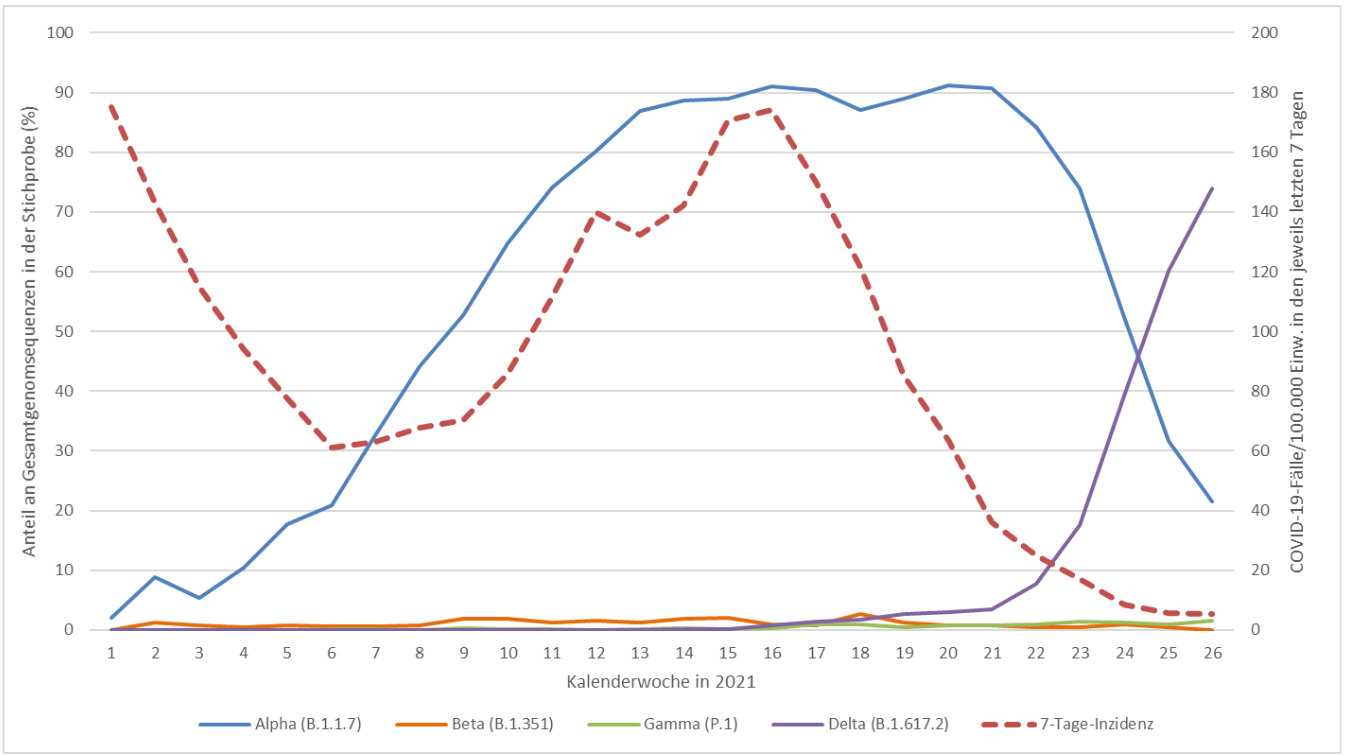
\includegraphics[width=1.0\linewidth]{figures/rkiVariantDistribution.png}
	\caption{Variant distribution in Germany over time \cite{robertkochinstituteditorBerichtVirusvariantenSARSCoV22021}}
	\label{rkiVariantDistribution}
\end{figure}

That is why we selected the data from 04.05.2021 (calendar week 18) until 15.07.2021 (calendar week 28). This results in a raw dataset of 35.818 genomes.
Each genome consists of a fasta file containing the genomes sequence and a record in a tsv file with the metadata.

TODO: beispiel record: genome sequence and metadata


\subsubsection{Generation of a phylogenetic tree}
\label{ch:approachAb}

As described above we need parent child genome sequence pairs to be able to train a \ac{ML} model. Therefore we need to evaluate the ancestral relationships between the genome sequences.
As described in chapter \ref{fundamentalsA0d} this is done in biology through phylogenetic trees.
For the data preparation (e.g. alignment) and the calculation of the phylogenetic tree we use the nextstrain pipeline \cite{10.1093/bioinformatics/bty407}.
The pipeline was executed on a local computer with Intel Core i7-7500U (4*2.70GHz), NVIDIA GeForce 940MX and 16 GB RAM.
Unfortunately after two days of calculation, the nextstrain pipeline exited with a out of memory exception. That is why the amount of data is decreased. This was done through iterative reduction of the dataset size. The largest locally computable dataset consists of 11.773 genome sequences.

The generated phylogenetic tree can be seen in figure \ref{phylogeneticTree}.
TODO: Beschreibung was man sieht

%TODO: nicer tree image?
\begin{figure}[ht]
	\centering
	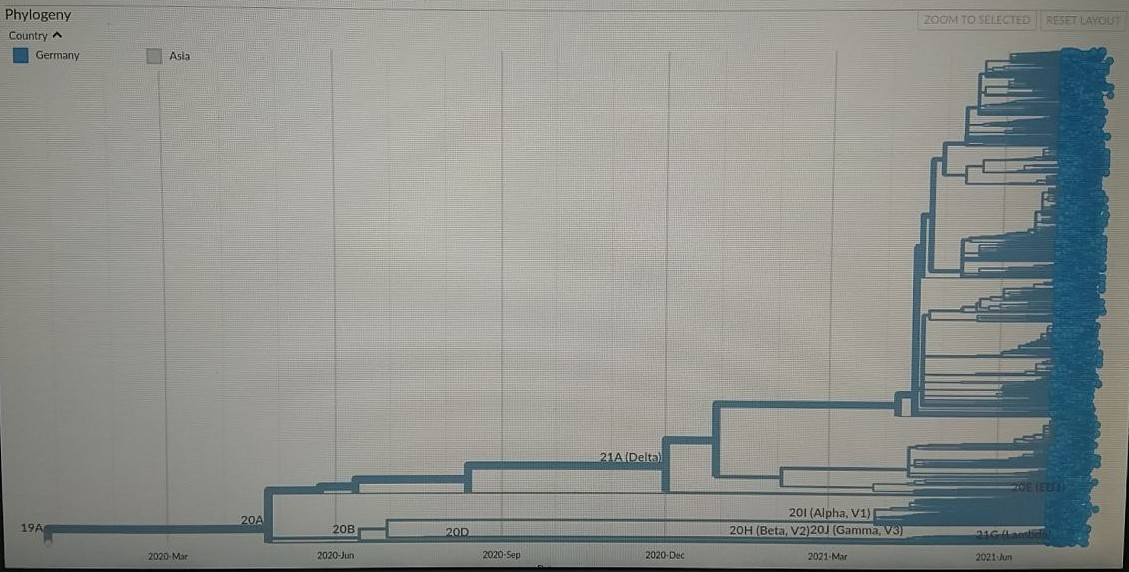
\includegraphics[width=1.0\linewidth]{figures/phylogeneticTree.jpg}
	\caption{Phylogenetic tree of our dataset \cite{own representation}}
	\label{phylogeneticTree}
\end{figure}

\subsubsection{Phylogenetic tree to dataset}
\label{ch:approachAc}

Based on the calculated phylogenetic tree the final dataset is generated. Therefore the patristic distances between all leaf nodes are calculated. From the resulting patristic distance matrix for each leaf node the most related next leaf node can be evaluated. The two leaf nodes with the smallest distance are the closest relatives to each other and therefore represent a parent child pair. After the evaluation which leaf nodes are one parent child pair, the question which node is the parent and which node is the child is clarified. Therefore the two nodes are sorted by their date, which is stored in the metadata file. The older genome sequence is the parent and the younger genome sequence is the child.

For calculating the patristic distance matrix we first used Dendropy (version: 4.5.2). Again this leads to problems due to limited RAM on our local computer. As a consequence we switched to PhyloDM (version: 1.3.1), which is a library for calculating patristic distances in a memory and time efficient manner.

Finally we received a dataset containing parent child genome sequences.

\subsection{Data Preprocessing}  \label{ch:approachB}
% TODO: Pipeline image
% Word size 3 is just a hyperparameter (see discussion of the corresponding paper)!  But maybe biologically valid because auf amino acids.
% DNA2Vec?

two steps:
- to make the dimensionality managable not the whole 30000 nucleotides are evaluated. We take a subpart of X nucleotides from position A to B
- Transform string to numeric for model input

\subsubsection{Dimensionality reduction by selecting subpart of the genome}
\label{ch:approachBa}


\subsubsection{Transform genome sequence to numeric model input}
\label{ch:approachBb}


\begin{itemize}
	\item DNA Sequencing (Done during dataset creation, given from GISAID)
	\item DNA Sequence Tokenization for Amino Acid Dictionary
	\item DNA Sequence Padding
\end{itemize}

\subsection{Model Architecture}  \label{ch:approachC}
% Hyperparameters and model architecture
% Reference http://nlp.seas.harvard.edu/2018/04/03/attention.html if one wants to build it by oneself

\subsection{Training Process} \label{ch:approachD}
% Plot accuracy and loss for training and validation
% Loss functions and teacher forcing, early stopping?
% Categorical cross-entropy loss for seq2seq, Wasserstein loss for GAN, kullback leibner + cross entropy for transformers
% Identify changes between sequences using the diff-match package from Google
% See MutaGAN 6.2 Model training
% Replay buffer
% Dealing with the mode collapse problem

\newpage
